%\documentclass[review]{elsarticle}
%
%\usepackage{lineno,hyperref}
%\usepackage{epstopdf}
%\usepackage{algorithm}
%\usepackage{algpseudocode}
%\usepackage{graphicx}
%\usepackage{multirow}
%\usepackage{amsmath}
%\usepackage{booktabs}
%\usepackage{color}
%\newcommand{ 	}{\textcolor{blue}}
%\PassOptionsToPackage{hyphens}{url}
%%\usepackage{breakurl}
%
%\modulolinenumbers[5]
%
%\journal{Journal of Parallel and Distributed Computing}
%
%
%
%%% `Elsevier LaTeX' style
%\bibliographystyle{elsarticle-num}
%%%%%%%%%%%%%%%%%%%%%%%%
%
%\newcommand{\black}{\textcolor{black}}
%%\newcommand{\blue}{\textcolor{blue}}
%
%
%%\hyphenation{Ho-we-ver}
%
%\begin{document}
%
%\begin{frontmatter}
%
%\title{Accelerating an algorithm for perishable inventory control on heterogeneous platforms}
%
%  \author[add1]{Alejandro Guti\'errez-Alcoba\corref{cor1}}
%  \ead{agutierreza@uma.es}
%  \author[add2]{Gloria Ortega}
%  \ead{gloriaortega@ual.es}
%  \author[add1]{Eligius M.T. Hendrix}
%  \ead{eligius@uma.es}
%  \author[add1]{Inmaculada Garc\'ia}
%  \ead{igarciaf@uma.es}
%
%  \cortext[cor1]{Corresponding author}
%  \address[add1]{Department of Computer Architecture, \black{Escuela de Ingener\'ias, c/ Dr Ramos,  University of} M{\'a}laga, M{\'alaga}, 29071, Spain}
%  \address[add2]{Informatics Department, University of Almer\'ia, Agrifood Campus of Int. Excell. (ceiA3), Almer{\'i}a, 04120, Spain}
%
%\begin{abstract}
%This paper analyses and evaluates parallel implementations of an optimization algorithm for perishable
%inventory control problems. This iterative algorithm has high computational requirements when solving large problems. Therefore, the use of \blue{parallel and distributed computing}  reduces the execution time and improves the quality of the solutions.
%This work investigates two implementations on heterogeneous platforms: (1) a MPI-PTHREADS version; and (2) a multi-GPU version. A comparison of these implementations has been carried out. Experimental results show the
%benefits of using \blue{parallel and distributed} codes to solve this kind of problems.
%
%Furthermore, the distribution of the workload among the available processing elements is a challenging problem. This distribution of tasks can be modelled as a Bin-Packing problem. This implies that the selection of the set of tasks assigned to every processing element requires  the design of
%a heuristic capable of efficiently balancing the  workload statically with no significant overhead. This heuristic has been used for the parallel implementations of the optimization for perishable
%inventory control problem.
%\end{abstract}
%
%\begin{keyword}
%Perishable inventory control, GPU computing, Heterogeneous computing,  Optimization, Monte Carlo simulation, Bin-Packing problem
%\end{keyword}
%
%
%\end{frontmatter}
%
%\linenumbers

\chapter{Accelerating an algorithm for perishable inventory control on heterogeneous platforms} % top level followed by section, subsection
\label{Chap:jpdc}

\section{Introduction}



The main objective of this work consists of determining up to what extent the use of heterogeneous platforms (multicore and multi-GPU) accelerates the solution process
of a novel optimization algorithm
for an inventory control problem of perishable products. Our goal is to study how to take advantage of the computing capacity of these architectures to obtain more accurate solutions when large problems are considered, which imply high computational demand, keeping a reasonable response time.






The perishable inventory control problem %\blue{
presented in this chapter %}
 is defined over a finite horizon of $T$ periods of a perishable product in which a fixed percentage of the non-stationary stochastic demand has to be satisfied according to a so-called fill rate service level requirement. The perishable product has a fixed shelf life of $J$ periods. In the modeling of this problem, it is supposed that $J<T$ and the dynamics of the inventory follows the FIFO issuance (first in, first out), in which the oldest product is issued first.
Items of age $J$ cannot be used in the next period and are considered waste. The goal is to %find what service level is optimal, in the sense of
minimize the cost related to the production, distribution, storage and waste. % which exceed the shelf life.
 \cite{GutierrezAlcoba:ICCSA2015} describes an algorithm based on Monte Carlo simulation of the demand, specifically designed to solve this problem. This algorithm is able to determine the optimal order policy and the corresponding order quantities efficiently. However, the computational burden grows exponentially in the time horizon.



Currently, extended High Performance Computing architectures are heterogeneous platforms composed of distributed memory systems, where every processing element (node) has a multicore architecture with a certain number of cores~\citep{Hennessy12}.
These heterogeneous platforms offer higher peak performance compared to traditional CPUs being both
energy and cost efficient. Nevertheless, programming for heterogeneous environments
is a tedious task and has a long learning curve.
In this context, parallel implementations should be modified in order to be executed over such heterogenous architectures. Therefore, it is necessary to have a
good knowledge of both, the algorithm to parallelize and the computational resources  used for the implementation ~\citep{Lastovetsky12}.
Furthermore, accelerators, such as GPUs, FPGAs, Intel Xeon Phi coprocessors and so on, can be included on these architectures.

%\blue{
Inventory control problems for perishable products have been studied since the seventies. Recently several new inventory models for controlling perishable items have appeared. For instance,~\cite{Laxmi2015} considers an inventory system for perishable products where demand follows a Poisson distribution, service interruptions, retrial demands and negative customers are considered. The study obtains a $(s, S)$ policy, i.e. an order is placed whenever inventory  drops below a level $s$. In \cite{PaulsWorm2015}, a MILP (Mixed-Integer Linear Programming) approximation for an or order up to level policy is presented. For practical cases, the solutions obtained by this approximation are less than 5\% higher than those obtained by the optimal policy. Authors in~\cite{Li2015} consider a joint dynamic pricing and inventory control policy for stochastic inventory and perishable products. They obtain the optimal dynamic policy by solving a Hamilton - Jacobi - Bellman equation. Authors in~\cite{Feng2016} study a joint pricing and a dynamic production policy for perishable items, with the addition that shortages are not allowed, deriving the optimal sales price and designing algorithms to compute them. However,
to the best of our knowledge, no study has been done with respect to the use  of heterogeneous platforms for computer-intensive inventory control models for deriving optimal order policies for perishable product inventory control. Related to the acceleration of the Monte Carlo simulation, required for the model described in this chapter, recent works can be found in the literature in order to efficiently compute this simulation on heterogeneous platforms~\cite{Hung:2016,Miranda29052016}. %}

%consider an inventory system for perishable products where demand follows Poisson distributions and considering service interruptions, retrial demands and negative customers. They obtain a $(s,S)$ policy (an order is set whenever inventory drops below $s$).


{\color{black}In this study, the algorithm} to solve the perishable inventory control problem has been implemented on Multi-GPU clusters, as an example of heterogeneous platforms. In a Multi-GPU cluster, there are several distributed memory nodes, where every node is composed of a shared memory multicore architecture and one or more GPUs. Each GPU has a separate memory space. Therefore, if data dependencies among GPUs occur,
communication via PCI-Express is needed. The main advantages of using Multi-GPU computing are as follows: (1) the use of massively parallel platforms (GPUs) facilitates speeding up the most computationally intensive tasks, because these devices have enough computational power to calculate vectorial computation schemes; and (2) when the problem to solve is large enough, several distributed memory nodes can be used (with/without GPUs). In the literature, heterogeneous computing has been used to accelerate the execution of a wide variety of numerical models ~\cite{GloriaConcurrency,Tabik2013}. For the inventory control problem, the use  of %\blue{
parallel and distributed
%}
  platforms improves the accuracy of the results; parallel computation allows executions with a larger number of simulations to solve a particular problem in a reasonable runtime.


The parallel computational model associated to this problem can be described in terms of a set of independent tasks. However, the computational burden associated to each task is different and therefore a workload balancing problem may appear when the workload is distributed in a blind way. The problem of assigning tasks to processing elements is well-known in the literature as the Bin-Packing problem~\citep{Garey:1979:CIG:578533}.
Because this problem is NP-hard, several heuristics have been developed to distribute the workload efficiently among the available platforms.

The rest of the chapter is organized as follows. Section~\ref{secdes} discusses the  perishable inventory control problem. In Section~\ref{Sec:AlgoritmoSecuencial},
the implemented sequential algorithm to solve the problem is outlined. Section~\ref{Sec:ImplParalelas} describes the details of the implemented parallel versions and several heuristics for distributing the workload among the available processing elements  are described and evaluated.
Section~\ref{Sec:ResultsJPDC} studies and analyses the results of running various implementations on heterogeneous platforms.
Finally, conclusions are drawn in Section~\ref{Sec:Conclusions}.

\section{Description of the model}
\label{secdes}
The basis of the implementations presented in this work is an algorithm developed in Matlab to solve a MINLP (Mixed Integer NonLinear Programming) problem,  \cite{GutierrezAlcoba:ICCSA2015}. The algorithm sets a schedule, along a finite number of periods $T$, for the quantities that must be provided of a  product in order to satisfy the demand under a $\beta$ service level requirement implying that for every period and in terms of the expected value, more than a fraction $\beta$ of the demand is satisfied.
This is equivalent to at most a fraction $(1-\beta)$ of demand is lost due to a stock-out. The shelf life of the product after which the product perishes and becomes waste is $J<T$ periods. Furthermore, items are served following a FIFO  rule: products are served starting from the oldest ones.


The optimization problem consists of finding the quantities of the product that must be provided at every period such that the restrictions are met and the value of the objective function is minimized.  %\blue{
These quantities have to be determined at the beginning of the planning horizon, following a static uncertainty strategy over demand: the order quantities have to be defined for all $T$ periods before realization of demand. If the decision maker is able to adapt the production over the periods as the demand is observed, one may use another strategy. An approach to this scenario is discussed in \cite{Gutierrez-Alcoba16}. %}

\noindent The model is specified as follows.


\smallskip\noindent\emph{Indices}\\
\begin{tabular}{ll}
	$t$ & period index, $t=1,\ldots,T$
	\\
	$j$ & age index, $j=1,\ldots,J$, with $J$ the shelf \\& life of the product\\
\end{tabular}


\smallskip\noindent\emph{Data}\\
\begin{tabular}{ll}
	$ \textbf{d}_t$ &
	\parbox[t]{13cm}{demand at every period following normal distributions with mean $\mu_t>0$ and} \\&
	 \parbox[t]{13cm}{variance $(cv\times \mu_t)^2$ given  by a coefficient of variation $cv$, equal at every period}\\
	$k$ & ordering cost, $k>0$\\
	$c$ & unit cost, $c>0$\\
	$h$ & holding cost, $h>0$\\
	$w$ & waste cost, can be negative, but $w>-c$\\
	$\beta$ & Required service level, $0<\beta<1$
\end{tabular}

%\noindent 5pt

\smallskip\noindent\emph{Variables}\\
\begin{tabular}{ll}
	$Q_t \ge 0$ & order quantity in period $t$.     $Q$ represents the vector $(Q_1,\ldots,Q_T)$\\
	$Y_t \in \{0,1\}$ & indicates if order takes place in period $t$.\\&  $Y_t= 1$ if and only if $Q_t>0$. \\&  $Y$ denotes  vector $(Y_1,\ldots,Y_T)$\\
	$\textbf{X}_t$ & lost sales at period $t$\\
	$\textbf{I}_{jt}$ & inventory of age $j$ at the end of \\& period $t$,
	$I_{j0}=0$, $\textbf{I}_{jt} \ge 0$, %\\& for
	$j=1,\ldots,J$.\\
\end{tabular}


\smallskip\noindent
The notation $E(\cdot)$ is used to express the expected value of a stochastic variable (in bold face) and $(\cdot)^+=max(\cdot,0)$.

\smallskip\noindent
The objective function to be minimized depends on the vector $Q=(Q_1,\ldots,Q_T)$ and can be defined as:
%
\begin{equation}
\label{eq:obj}
f(Q)=\sum_{t=1}^T \left(C(Q_t) + E\left(h\sum_{j=1}^{J-1} \textbf{I}_{jt}  +w\textbf{I}_{Jt}\right)\right),
\end{equation}
where
\begin{equation}
\label{eq:proc}
C(x) = k+cx, \ \ \text{if} \ \ x>0,\ \text{and}\ \ C(0)=0 .
\end{equation}
%
The inventory of products of age $j$ at the end of period $t=1,\ldots,T$ follows the FIFO rule:
%
\begin{equation}
%\small
\label{eq:invWaste}
\textbf{I}_{jt}=
\begin{cases}
\left(Q_t - (\textbf{d}_t-\sum_{j=1}^{J-1}\textbf{I}_{j,t-1})^+\right)^+ & j=1,\\
(\textbf{I}_{J-1,t-1} - \textbf{d}_t)^+ & j=J, \\
\left(\textbf{I}_{j-1,t-1} - (\textbf{d}_t-\sum_{i=j}^{J-1}\textbf{I}_{i,t-1})^+\right)^+ & Otherwise\\
%& ,J-1 \
\end{cases}
\end{equation}
The service level requirement can be expressed as:
%
\begin{equation}
\label{eq:chance}
E \left(\textbf{X}_t\right) \le (1-\beta) \mu_t, \ t=1,\ldots,T.
\end{equation}
The value of  the lost sales in each period $t$ is given by:
%
\begin{equation}
\label{eq:lostsales}
\textbf{X}_t=\left(\textbf{d}_t-\sum_{j=1}^{J-1}\textbf{I}_{j,t-1}-Q_t\right)^+.
\end{equation}
%
The expected value of the lost sales is a function known as the \emph{loss-function}, that in general does not have a closed-form expression. Some approximations to this function can be found in the literature in \cite{kurawarwala96,Rossi14,DeSchrijver20121375,Waissi199691}.
Monte Carlo simulation  has been used for this model in order to obtain a good estimation of the \emph{loss-function}.
Having set the conditions detailed before, the problem of finding the quantities that have to be ordered to minimize the objective function \eqref{eq:obj} and at the same time finding the timing vector $Y\in \{0,1\}^T$ for the optimal policy, is a MINLP (Mixed Integer NonLinear Programming) problem. As will be shown, the  computational model associated to this problem exhibits appropriate properties for being implemented on heterogeneous high performance computers architectures.

\section{Sequential algorithm}
\label{Sec:AlgoritmoSecuencial}

This section describes the  algorithm for solving the inventory control problem of Section~\ref{secdes}. Algorithm  \ref{alg:bestY} represents the highest level of abstraction for the solution method. Firstly, the method generates all timing vectors  in  set $\{0,1\}^T$ that are feasible for the values of $T$ and $J$. A timing vector $Y\in \{0,1\}^T$ is considered infeasible if it contains a series of more than $J$ sequential zeros ($J$ or more periods without placing an order), since demand cannot be met. For a specific timing vector $Y$, Algorithm  \ref{alg:optimalforY} determines, for each period, the order quantity of product $Q(Y)$ that minimizes objective function \eqref{eq:obj}.


Algorithm \ref{alg:bestY} performs an exhaustive evaluation over the set of feasible timing vectors (except for the cases discarded by the lower bound check), to find the optimal timing vector  $Y^*$ and, at the same time, the vector of the optimal order quantities $Q^*=Q(Y^*)$ with associated cost $f(Q^*)$. Each vector $Y$ is composed of a number of cycles: a cycle is a set of periods in which a replenishment is set in the first period of the cycle, to cover the demand for all periods of the cycle. In any vector $Y$, a cycle is identified by a period with value 1 and a sequence of zeros from none to $J-1$.

\begin{algorithm}[hbt!]
\caption{$AllY()$: Finds the optimal timing vector ($Y^*$) calculating the optimal cost of all feasible timing vectors $Y$}
\label{alg:bestY}
\begin{algorithmic}[1]
%\Procedure{AllY}{ }
\STATE Generate all feasible $Y$
\FOR{all $Y$}
\STATE $Q_Y$=MINQ(Y); \# Algorithm \ref{alg:optimalforY} \label{bestY:line:NLPsolverJPDC}
\STATE Determine $f(Q_Y)$
\ENDFOR
\RETURN $Y^*$; $Q^*$; $f(Q^*)=$ mincost
\vskip 5pt
\end{algorithmic}

\end{algorithm}

For the determination of the optimal quantities, $Q(Y)$, the method uses a table of so-called base order quantities $\hat{q}_{R,t}$ with the required quantity at period $t$ to cover the demand of a cycle of $R$ periods when inventory is zero. This quantity is the order quantity for those order periods where no inventory is available. Let $m=\sum Y_t$ be the number of orders, then Algorithm \ref{alg:optimalforY} starts by identifying $m$-dimensional vector $A$ with the order moments and vector $B$ with the last period of each  cycle.
%
\begin{algorithm}[hbt!]
	\caption{$MinQ(Y)$: $Q(Y)$ optimization}
	\label{alg:optimalforY}
	\begin{algorithmic}[1]
		\STATE Generate vectors $A$ and $B$ for $Y$
		\FOR{$i=1$ \textbf{to} $m$}
		\IF{$A_i=1$ \textbf{or} $B_{i-1}-A_{i-1}=J$} %\# No Invent. 		
		\STATE $Q_{A_i}=\hat{q}_{(B_i-A_i),A_i}$
		%\STATE $floss(Q_i,A_i,A_i+R_i-1)$ \label{optimalforY:line:floss} \#Alg \ref{alg:simulation}
		\ELSE
		\STATE \textbf{solve} $floss(Q_{A_i},A_i,B_i)=(1-\beta)\mu_{B_i}$
		%\label{oldalg}
		%\STATE $Q_i=OrdVal(A_i,A_i+R_i)$ \# Alg~\ref{alg:ordervalue}
		\ENDIF
		\ENDFOR
		\RETURN $Q$;
		\vskip 5pt
	\end{algorithmic}	
\end{algorithm}


For each replenishment period, that is, any period $t$ in which $Y_t=1$, Algorithm \ref{alg:optimalforY} calculates the minimum order quantity that guarantees that the service level is fulfilled for that cycle. For each cycle, the optimal order quantity $Q_{A_i}$ is the one that makes that the lost sales are equal to the lower bound of (\ref{eq:chance}) in period $B_i$.
%
When there is no inventory, $Q_{A_i}$ can be taken as the base quantity \citep{GutierrezAlcoba:ICCSA2015}. When inventory is not zero,
Monte Carlo simulation of the  inventory is used to give an accurate approximation.  Function \emph{floss$(q,a,b)$} in Algorithm ~\ref{alg:simulation} handles the simulation  and returns the approximation of the expected value of lost sales for the last period of the cycle when $q$ units are ordered at period $a$ for a cycle with $(b-a)+1$ periods. An external function, like the secant method in  \cite{GutierrezAlcoba:ICCSA2015}, can iteratively look for the value of $q$ for which (\ref{eq:chance}) is fulfilled with equality.



\begin{algorithm}[hbt!]
	\caption{$floss(q,a,b)$: Monte Carlo method approximating $E(\textbf{X})$ based on $N$ sample paths $d_{t,n}$ }
	\label{alg:simulation}
	\begin{algorithmic}[1]
		%\Require Cantidad de pedido ($q$), periodos $[t_1,t_2]$, n�mero de simulaciones $N$%, fixed shelf life ($J$)
		%, inventario inicial $I_{jn}, j=1,\ldots,J-1, n=1,\ldots,N$%, $\mu_t, t\in[t_1,t_2]$, $cv$
		%\Ensure  Estimate $Z$ of $E(X_{t_2})$, a sample of $I_{t_2}$
		\FOR{$n=1$ \textbf{to} $N$}
		%\hfill \#Update inventory ($I$)
		\STATE \text{Simulate} $I_{j,t,n}$, $t=a,\ldots,b; \ j=1,\ldots,J$
        %\STATE %$x_b+= \left(d_{b,n}-\sum_{j=1}^{J-1}I_{j,b-1,n}-q\right)^+$;
        \STATE $x_{bn}$ loss in sample $n$ at end period $b$, $\sum\limits_{n=1}^Nx_{bn}$
        \ENDFOR
        \STATE Average loss $X_b=\frac{1}{N}\sum\limits_{n=1}^Nx_{bn}$ approximates $E(\textbf{X})$
		\RETURN $X_b$;
	\end{algorithmic}
\end{algorithm}

\section{Parallel implementations}
\label{Sec:ImplParalelas}

The order of complexity of Algorithm~\ref{alg:bestY}, is related to the number of feasible timing vectors $Y$, which depends on the values of $J$ and $T$.
Independently of the value of $J$, the number of feasible cases to process increases
exponentially with the value of $T$. This means that the complexity is  $O(e^T)$. Moreover, in Algorithm~\ref{alg:optimalforY}, the optimal value of the $Q(Y)$  vector is found for a specific feasible $Y$; its complexity depends on the number of iterations needed to solve the equation in line 6 which is bounded by $T$. Evaluation of $floss$ in Algorithm~\ref{alg:simulation} (Monte Carlo simulations) requires $N$ simulations of the inventory for every period in the cycle and all possible ages of the product ($1, \ldots,J$).
%


Therefore, the order of complexity of the whole method  to find the
 optimal timing vector $Y$ and the optimal quantities, is approximately $O(N \cdot T \cdot e^T)$.

Algorithm \ref{alg:simulation} requires simulation to obtain approximations of the ~\emph{floss} function.
This function consumes most of the computational runtime of the algorithm.
A higher number of demand paths in the Monte Carlo simulation provides more accurate approximations of the lost sales (\emph{floss} function). The standard deviation of the estimate std$(\boldsymbol{X_b})$ reduces with $N$ according to std$(\boldsymbol{X_b})=\frac{\text{std}(\boldsymbol{x_{bn}})}{\sqrt N}$. Figure~\ref{fig:hist} shows the density distribution of estimating the percentage of lost sales $\boldsymbol{X_b}$, when $\boldsymbol{X_b}$ is estimated based on  $N=20000, 30000, 50000$ sample paths for a case that analytically gives the value $\frac{E(\boldsymbol{X_b})}{\mu_b}=0.05$, that is, the lost sales is 5\% of the expected demand $\mu_b$.


Therefore, approximating the expected lost sales ($X$) accurately requires a  sufficiently high number $N$ of sample paths. This represents the main computational workload of the problem.

\begin{figure}
\centering
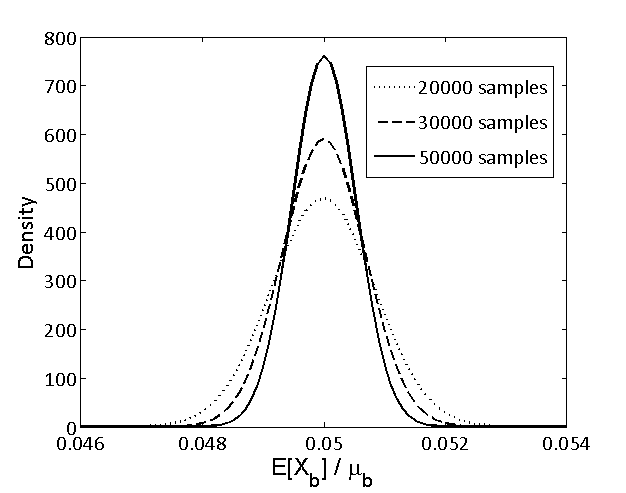
\includegraphics[scale=0.5]{jpdc/figures/figure1paper.png}
\caption{Density functions of the estimation of the percentage of the expected value of $\frac{X_b}{\mu_b}$ according to the Algorithm \ref{alg:simulation} using $N=20000, 30000, 50000$ sample paths}
\label{fig:hist}
\end{figure}

From a parallel point of view, Algorithm~\ref{alg:bestY} can be decomposed into independent tasks, as  there are hardly dependencies in the computation associated to each $Y$. So, the loop ``for" in Algorithm~\ref{alg:bestY} can be executed in parallel. However, the computational burden associated to each $Y$ is different and requires distributing vectors $Y$ among the available processing elements in a balanced way. To do that, an estimation of the workload for each $Y$ is needed.

The workload associated to a feasible timing vector $Y$ (Algorithm~\ref{alg:optimalforY}) can be estimated. In this way the most time-consuming task of this approach (the Monte Carlo simulations) can be taken into account to find the optimal solution. More precisely, the Monte Carlo simulation for an order depends on the length of the replenishment cycle which varies between $1$ and $J$ periods. Following Algorithm \ref{alg:optimalforY}, for cycles in which there is no left inventory, the quantity of product needed  is already known from the so called basic quantities. After that, only one Monte Carlo simulation must be carried out. For any other period, an external function iteratively performs Monte Carlo simulation up to a certain accuracy. With the method used in \cite{GutierrezAlcoba:ICCSA2015}, the number of iterations of Algorithm \ref{alg:simulation} needed to solve the equation line 6 of Algorithm \ref{alg:optimalforY} depends on the accuracy chosen and an average value of $K$ iterations can be assumed. The workload of any vector $Y$ can be taken as the accumulation of Monte Carlo simulations per period that are needed, as sketched in Algorithm~\ref{alg:rankY}.

  \begin{algorithm}[hbt!]
  	\caption{$Rank(Y)$: Workload approximation for $Y$}
  	\label{alg:rankY}
  	\begin{algorithmic}[1]
  	
  		\STATE Generate vectors $A$ and $B$ for $Y$
  		\FOR{$i=1$ \textbf{to} $m$}
  		\STATE $length\_cycle=B_{i-1}-A_{i-1}$;
  		\IF{$A_i=1$ \textbf{or} $length\_cycle=J$} %\# No Invent. 		
  		\STATE $v+=length\_cycle$;
  		%\STATE $floss(Q_i,A_i,A_i+R_i-1)$ \label{optimalforY:line:floss} \#Alg \ref{alg:simulation}
  		\ELSE
  		\STATE $v+=length\_cycle \cdot K$
  		\label{oldalg}
  		%\STATE $Q_i=OrdVal(A_i,A_i+R_i)$ \# Alg~\ref{alg:ordervalue}
  		\ENDIF
  		\ENDFOR
  		\RETURN $v$;
  		\vskip 5pt
  		
  	\end{algorithmic}	
  \end{algorithm}





Now that the parallel decomposition of the problem has been analysed, the details of the implemented approaches are described in the following sections. Section~\ref{sub:MPI-PTHREADS} describes the computational platform and programming interfaces for the MPI-PTHREADS implementation and Section~\ref{sub:GPU} gives the Multi-GPU implementation.  In Section~\ref{SubSec:BinPacking}, the heuristics used to distribute the workload among processing elements are discussed.  Implementations described in~\ref{sub:MPI-PTHREADS} and ~\ref{sub:GPU}  have been carried out on a heterogeneous platform which consists of a multi-GPU cluster (composed of several nodes with multicores and GPU devices). The exploitation of a heterogeneous platform has two main advantages: (1) larger problems can be solved; and (2) it can be done in less runtime.
\begin{itemize}
	\item{MPI-PTHREADS:} obtains the parallelism of the nodes and the multicore processors available in the cluster.
Therefore, programming with POSIX Threads (pthreads~\footnote{\url{https://computing.llnl.gov/tutorials/pthreads/}})  and distributed programming based on Message Passing Interface (MPI) are used~\citep{pthreads,MPI}.
	\item{Multi-GPU:} uses GPUs in order to parallelize the Monte Carlo simulation, which is the most computationally demanding task of the problem. For this, the CUDA~\footnote{\url{https://developer.nvidia.com/cuda-toolkit}}  interface is used. In this case the implementation uses MPI and CUDA.
\end{itemize}



\subsection{MPI-PTHREADS implementation}
\label{sub:MPI-PTHREADS}
Focusing now on the MPI-PTHREADS implementation, parallelism has been exploited on two  levels: at node level (distributed memory) and at multicore level (shared memory).
On one hand, at node level, and thanks to its portability, Message Passing Interface (MPI)~\citep{MPI}
has become a standard for multiple-processor programming of code that runs on a variety of machines.
On the other hand, there are multiple ways of parallelizing routines in shared memory models. One standard library is POSIX threads
(or Pthreads), which supplies a unified set of C routines  facilitating the use of threads in  codes~\citep{pthreads}.

A hybrid parallelization (MPI and Pthreads) of the optimization algorithm for perishable inventory control problem described in Section~3 has been implemented.
At the beginning of Algorithm~\ref{alg:bestY}, the set of timing vectors $Y$ are distributed among cores following the rules of a heuristic designed  for balancing the workload which is discussed in Section~\ref{SubSec:BinPacking}. This MPI-PTHREADS implementation has been tested in a Bullx cluster and obtained results are described in Section~5.



\subsection{Multi-GPU implementation}
\label{sub:GPU}
The Multi-GPU version has been based on the exploitation of several GPUs for the parallelization of the Monte Carlo method, computed by the \emph{flossGPU} function (see Algorithm~\ref{alg:cuda}). In this implementation, each MPI process can open one or two threads and every thread initializes the CUDA interface. Timing vectors $Y$ are distributed among cores in the same way as in the MPI-PTHREADS implementation (following the rules of a heuristic designed  for balancing the workload which is discussed in Section~\ref{SubSec:BinPacking}).
Only Monte Carlo simulations are computed on the GPU, the remaining tasks are computed by the CPU (cores).
  The $N$ sample paths in the Monte Carlo simulation have been implemented to run independently. At the same time, the calculation of the inventory level at each age~(\ref{eq:invWaste}) depends only on the inventory level of the previous period. Then, proceeding by periods, a CUDA kernel is responsible to compute $N$ simulations of the $J$ ages of the inventory in parallel.

In Algorithm~\ref{alg:cuda}, Monte Carlo simulation ($flossGPU$ function) is performed on one or several GPUs.
The external loop simulates the periods, while the inner loop computes $N$ samples on the GPU.
This way, each GPU launches $N$ threads in parallel, computing the same sequence of instructions over
different input data. Thus, the programmer can consider the GPU as a set of SIMT (Single Instruction, Multiple Threads).
Each GPU thread stores its partial computation in the shared memory. To generate the approximation of $X$, one
reduction of the $N$ values computed and stored in shared memory has to be included.
One additional issue has been the optimization of the occupancy on the GPU. The occupancy determines how
well the hardware is kept busy with the goal of hiding
latencies, by switching between active warps, due to memory
operations and paused warps.
Occupancy is closely related
to the thread block size ($BS$) and the number of registers and
shared memory size used by a kernel. Therefore, a good choice
of $BS$ will improve the performance. Experimental results of Section~\ref{Sec:ResultsJPDC} have considered the best $BS$ size (512) to optimize the performance of the GPU code.


Section~\ref{Sec:ResultsJPDC} presents the experimental results of both implementations, MPI-PTHREADS and Multi-GPU.


\begin{algorithm}[bt!]
    \caption{$flossGPU(q,a,b)$: Monte Carlo method for obtaining an approximation of  $E(\textbf{X})$}
    \label{alg:cuda}
    \begin{algorithmic}[1]
        \FOR{$t=a$ \textbf{to} $b$}
        \FOR{$n=1$ \textbf{to} $N$} % \#GPU %(lines 2--5)
        \STATE Update $I_{j,t,n}$, $j=1,\ldots,J$ and $x_{tn}$
        %\STATE $x_b+= \left(d_{b,n}-\sum_{j=1}^{J-1}I_{j,b-1,n}-q\right)^+$;
        \ENDFOR
        \ENDFOR
        \STATE Average loss $X_b=\frac{1}{N}\sum\limits_{n=1}^Nx_{bn}$ approximates $E(\textbf{X})$
        %\STATE $X_b=\frac{x_b}{N}$
        \RETURN $X_b$;
    \end{algorithmic}
\end{algorithm}
%%%%%%%%%%%%%%%%%%%%%%%%%%%%%%%%%%
\subsection{Heuristics for the Bin-Packing problem}
\label{SubSec:BinPacking}


The problem for distributing the workload of Algorithm~\ref{alg:bestY} among processors can be modelled as a Bin packing problem. The Bin-Packing problem is a combinatorial optimization problem (NP-complete) and for the inventory problem it can be described as  follows: Given a set of $L$ independent runs  of the same algorithm with workload  $0< w_i < C$, $i=1,\ldots, L$, for each independent run $i$ of Algorithm  \ref{alg:optimalforY} (the feasible timing order vectors) and a set of $P$ processors (Bins), distribute the runs of the algorithm among the processors $p=1,\ldots,P$ such that the maximum workload assigned to a processor is as low as possible. See~\cite{Garey:1979:CIG:578533} for a general formulation of the Bin-Packing problem.


Due to the hardness of finding optimal solutions for this kind of problems, some heuristics capable of finding acceptable solutions in a reasonable time are usually considered, some of them are based on evolutionary computation, e.g. ~\cite{Blum:2003:MCO:937503.937505}. Here we have tested three heuristics (H1, H2 and H3) which are able to provide approximate solutions to the workload balancing problem.
 These heuristics attempt to distribute the workload $w_i$ equally  over the available cores.
%
\begin{enumerate}
	\item (H1) is based on Round Robin scheduling: Sort $w_i$ from high to low and assign to $p$ following the pattern  $(1,\ldots,P,P,P-1,\ldots,1,1,\ldots)$.
	\item (H2): For $i=1,\ldots,L$ assign $w_i$ to processor $p$ with the lowest gathered workload.
	\item (H3): Similar to heuristic H2, but in this case $w_i$ is sorted previously from high to low values.
\end{enumerate}

To evaluate the heuristics, three  instances called $\Gamma_1$, $\Gamma_2$ and $U$ where generated by taking $L=4000$ weights $w_i$ at random from gamma distributions $\Gamma(10,4)$ and $\Gamma(1,25)$ and from the uniform distribution $U(0,100)$, respectively. Moreover, an instance $\Delta$ was taken from a real workload distribution of the inventory control problem with $T=15$ and $J=3$. Figure \ref{fig:gam} sketches the corresponding distributions.


\begin{figure}[hbt!]
	\centering
	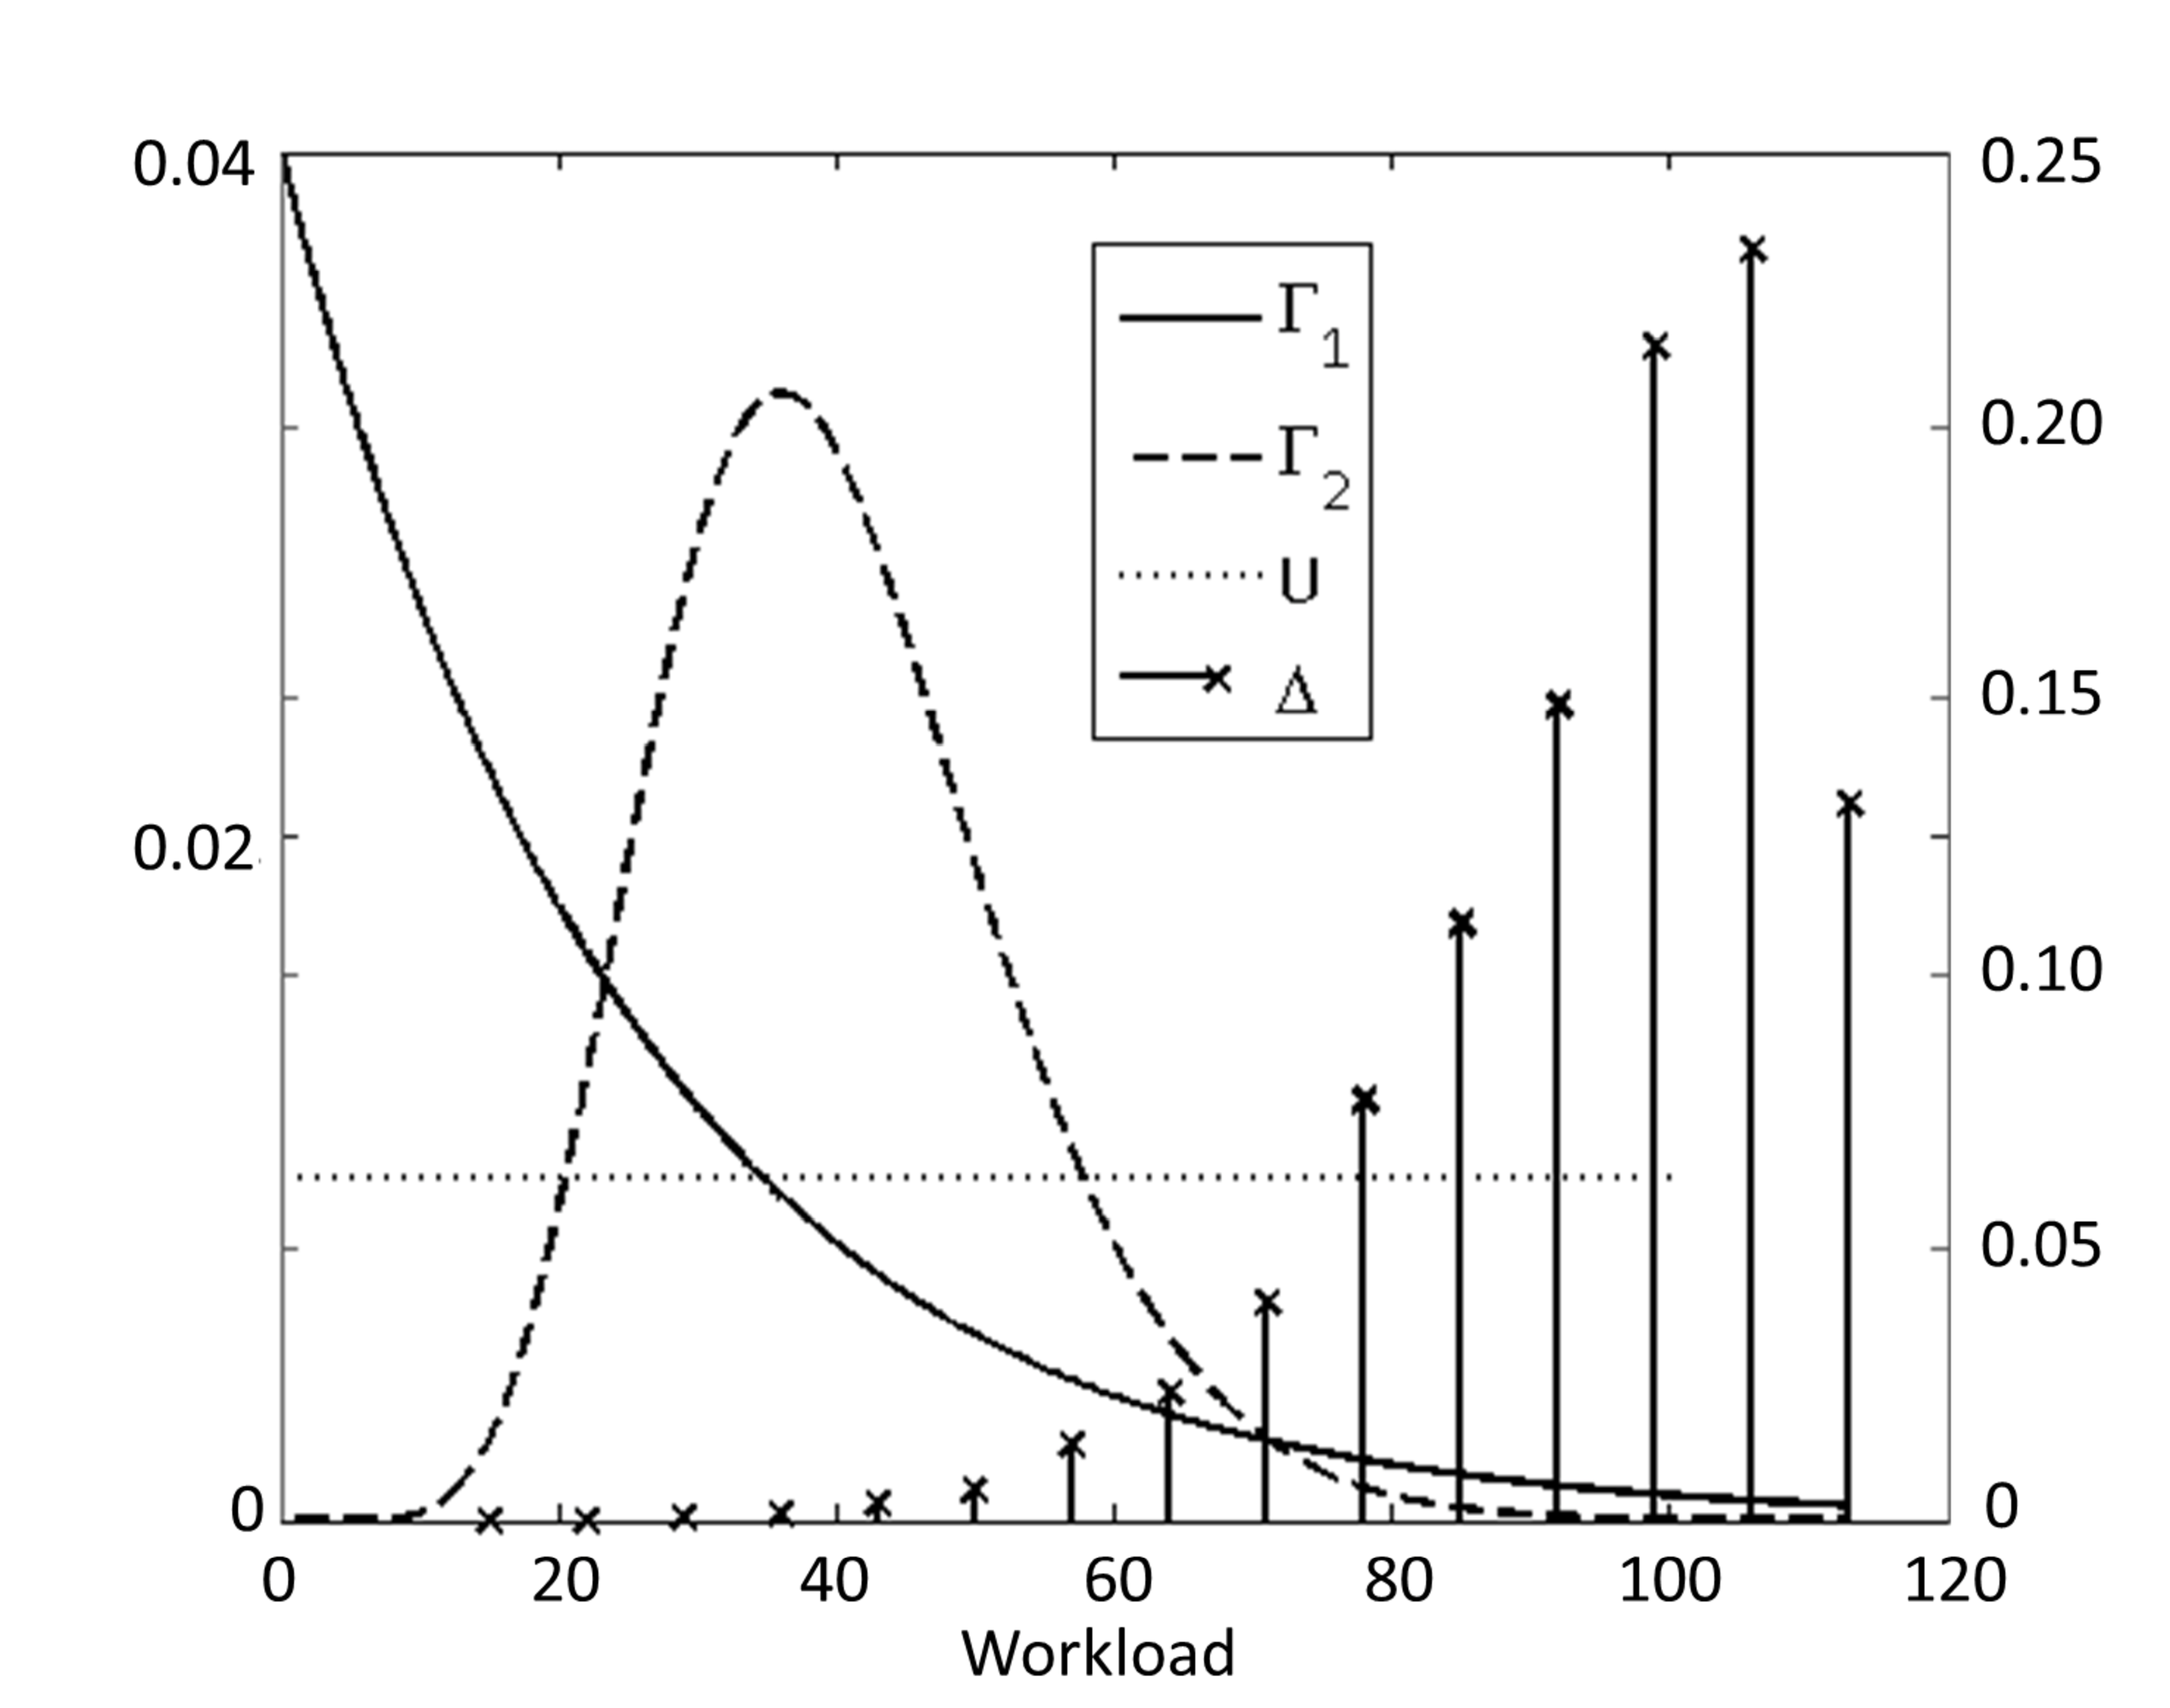
\includegraphics[scale=0.16]{jpdc/figures/figure2.pdf}\\
	\caption{Probability density functions of  $\Gamma (10,4)$, $\Gamma(1,25)$, $U(0,100)$ used to generate the 4000 samples combined with the distribution of the inventory instance, $\Delta$. }
    \label{fig:gam}
\end{figure}

To calculate the workload balancing assigned to each processor, the coefficient of Gini ($G$) \cite{Gini0}
has been used in this work following the examples in~\cite{Gini1,Gini2,Gini3}. This coefficient has been  widely used in economy to measure the degree of inequality and wealth distribution for large populations. The Gini index varies between 0 representing complete equity and 1 if all the wealth (workload) of the population belongs to only one individual (processor)~\cite{Gini0}. Let  $W_p$ be the workload assigned to processor $p$, $p=1,\ldots,P$ sorted in ascending order. The Gini coefficient $G$ is:
%
\begin{equation}
	G= \frac{2\sum\limits_{p=1}^{P} p W_p}{P\sum\limits_{p=1}^{P}W_p}-\frac{P+1}{P}
\end{equation}

Table~\ref{tab:heurperformance} summarizes the behaviour of the heuristics, considering the Gini coefficient ($G$) for the samples (compared to a blind distribution of the workload (HR column)). Clearly, this table shows that heuristic H3 is, at least, better than heuristics H1 and H2 in an order of magnitude, and that a random workload assignment (HR) is at least two orders of magnitude worse than H3 and one for H1 and H2. From the data in Table~\ref{tab:heurperformance}, can be concluded that heuristic H3 presents the best results, being able to balance the workload almost perfectly.

\begin{table}[hbt!]
	
	\caption{Gini coefficient in $10^{-6}$ of the workload distribution of heuristics H1, H2 and H3 versus a random allocation HR.   $P= 8,16,32,64$, weights $w_i$ from  $\Gamma_1$, $\Gamma_2$ and uniform distribution, $\Delta$ is an empirical distribution.}
    \label{tab:heurperformance}
    \centering
    \small
	\begin{tabular}{crrrrr}
		\toprule
    & \multicolumn{1}{c}{$P$} & \multicolumn{1}{c}{H1} &\multicolumn{1}{c}{H2} & \multicolumn{1}{c}{H3} & \multicolumn{1}{c}{HR} \\ \midrule
	\multirow{4}{*}{$\Gamma_1$}	& $8$  &  $130$        	& $480$      	& $12$         & $3700$        \\
		& $16$ &  $250$         	& $1200$      	& $52$         & $7600$        \\
		& $32$ &  $580$          & $2000$      	& $140$         & $13000$        \\
		& $64$ &  $3200$          & $3900$      	& $1500$         & $21000$       \\ \midrule
&\\%%%%%%%%%%%%%%%%%%%%%%%%%%%%%%%%%%%%%%%%%%%%%%%		
	\multirow{4}{*}{$\Gamma_2$} &	$8$  	&  $690$        	& $1000$      	& $19$         & $23000$        \\
		& $16$ 	&  $1200$         	& $2100$      	& $19$         & $39000$        \\
		& $32$ 	&  $3300$          & $4100$      	& $78$         & $61000$        \\
		& $64$ 	&  $8000$          & $7600$      	& $100$         & $79000$         \\	\midrule
&\\%%%%%%%%%%%%%%%%%%%%%%%%%%%%%%%%%%%%%%%%%%%%%%%		
	\multirow{4}{*}{U} &	$8$  	&  $130$        	& $750$      	& $7.4$         & $12000$   \\
		& $16$ 	&  $180$         & $1400$      	& $8.6$         & $18000$        \\
		& $32$ 	&  $220$         & $2400$      	& $39$         & $26000$        \\
		& $64$ 	&  $370$         & $4100$      	& $54$         & $40000$        \\	\midrule		
	\multirow{4}{*}{$\Delta$} &	$8$  	&  $43$        	    & $190$      	& $30$         & $3200$   \\
		& $16$ 	&  $220$         & $460$      	& $230$         & $4500$        \\
		& $32$ 	&  $300$         & $1000$      	& $320$         & $7100$        \\
		& $64$ 	&  $550$         & $2000$      	& $380$         & $9800$        \\	\bottomrule		
	\end{tabular}
\end{table}





\section{Experimental results}
\label{Sec:ResultsJPDC}
For the evaluation of the implementations of Algorithm \ref{alg:bestY} to solve the perishable
inventory control problem, a Bullx cluster composed of eight nodes with a total of 128 cores has been used. In particular,  each node contains two Intel Xeon E5 2650 and a total of 16 cores. The eight nodes are interconnected by a QDR/FDR InfiniBand port embedded on the motherboard. Four of the nodes have two GPUs (total of $2\times4$ NVIDIA Tesla M2070). The main characteristics of the GPUs
are described in Table~\ref{Tab:charGPU}. The experiments have been compiled
with NVIDIA CUDA (6.5 version),  %\blue{
gcc compiler (4.8.1 version) with -O2 as the optimization option and OpenMPI as the MPI library. %}


\begin{table}[hbt!]
    \caption{Characteristics of the GPUs considered for the evaluation.}
    \centering	
    \label{Tab:charGPU}
    \begin{tabular}{rr}
    \toprule
               & Tesla M2070 \\ \midrule
    Peak performance (double prec.) (GFLOPs) &     515 \\
    Peak performance (simple prec.) (GFLOPs) &     1030 \\
    Device memory (GB) &       5.24 \\
    Clock rate (GHz) &        1.2 \\
     Memory bandwidth (GBytes/sec )  &     150 \\
    Multiprocessors &         14 \\
    CUDA cores &        448 \\
    Compute Capability &          2 \\
     DRAM TYPE &      GDDR5 \\ \bottomrule
    \end{tabular}
\end{table}

In order to test the parallel implementations, an inventory control problem of perishable products based on $T=15$ and $J=3$ has been considered.
It comprises a total of $L=5768$ feasible timing vectors $Y$.
For Monte Carlo simulation, $N=200000$ samples are used in Algorithm~\ref{alg:simulation}.

Figure~\ref{fig:MPIPthreadsorder} illustrates the values of the execution time for the MPI-PTHREADS implementation using 1, 2, 4, 8 and 16 threads and 1, 2, 4 and 8 MPI processes. A maximum of eight nodes has been considered. At every node, only one MPI process is executed and the number of Pthreads launched per node varies from 1 to 16 (one thread per physical core). The number of cores $P$ in which the heuristic balances the workload associated to $L$ feasible timing vectors $Y$ of the problem is equal to the number of MPI processes $\times$ the number of threads.




\begin{figure*}[hbt!]
\centering
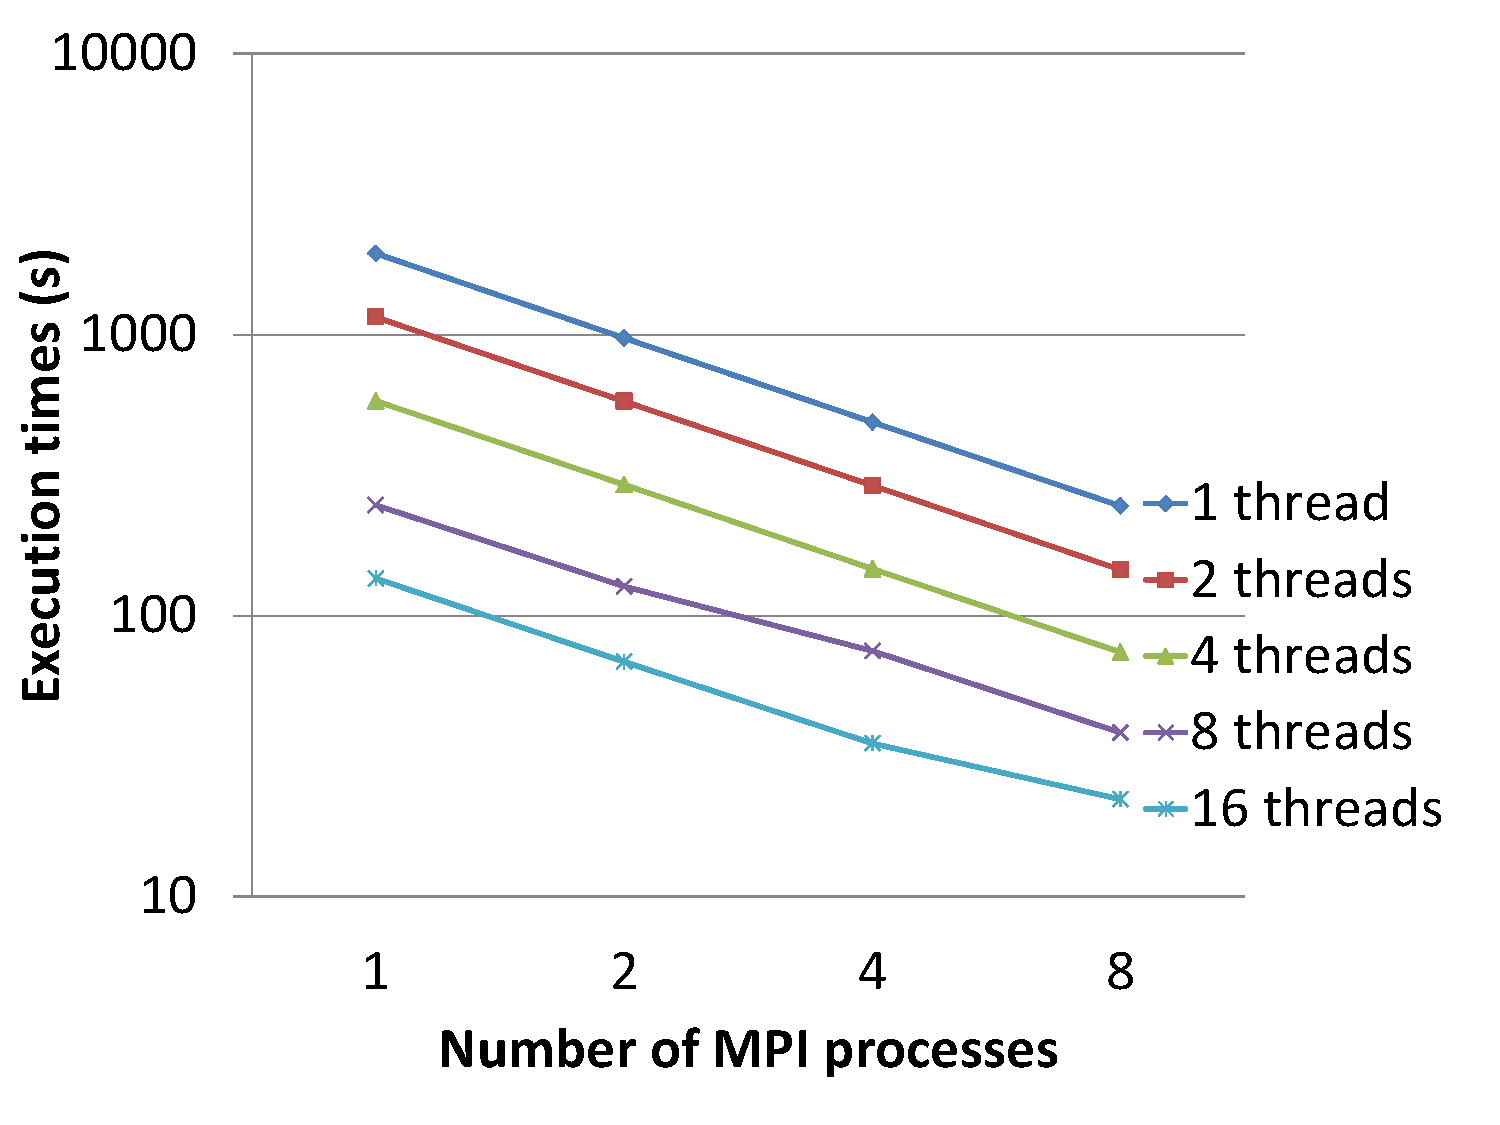
\includegraphics[scale=0.3]{jpdc/figures/MPIPthreadsorder.pdf}
\caption{Executions time, in seconds, of the MPI-PTHREADS implementation using H3 heuristic. }
\label{fig:MPIPthreadsorder}
\end{figure*}


Figure~\ref{fig:SpeedUpMPIPthread} shows the speed up of the MPI-PTHREADS implementation using H3 ranging from $1.7$ for the version with
a single MPI process with 2 threads to $87.5$ for 8 MPI processes with 16 threads each. The performance increases with the number of MPI processes. So, the best
results in terms of performance are obtained for 8 MPI (8 nodes). The Y-axis of the figure highlights how the number of threads in a MPI process affects the total performance of the algorithm. To be more precise, for the same number of MPI processes, duplication of the number of threads (and cores) offers an acceleration factor of nearly $2$.

\begin{figure*}[bt!]
\centering
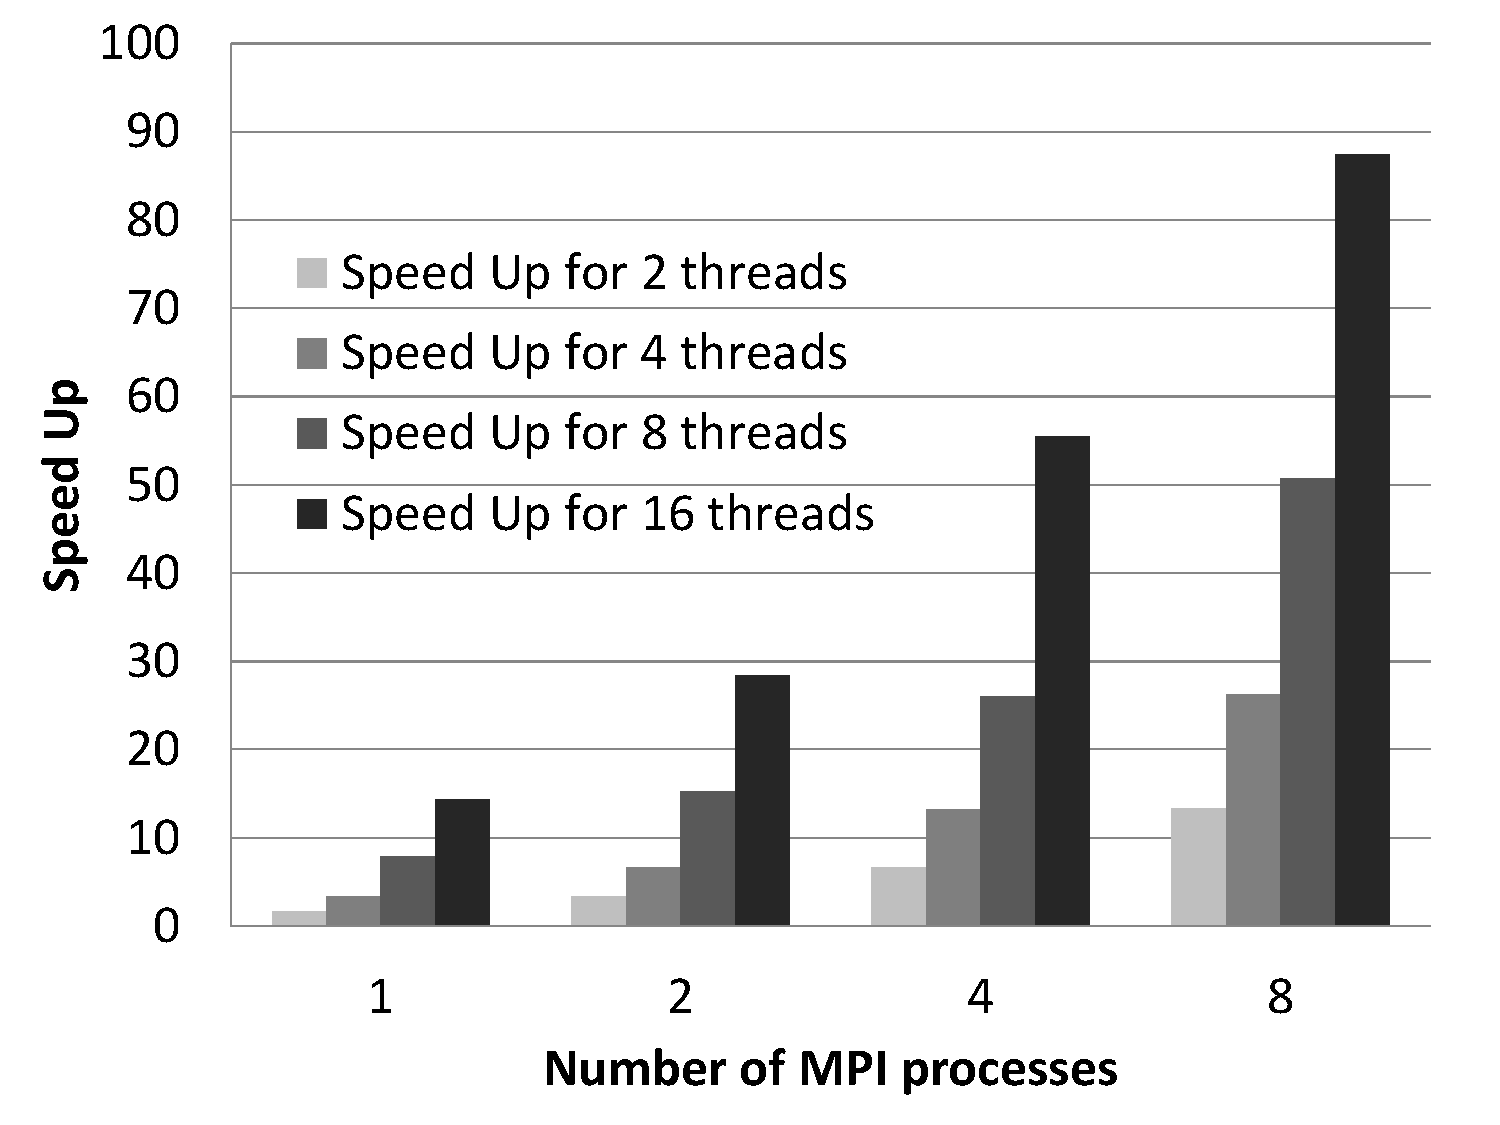
\includegraphics[scale=0.3]{jpdc/figures/SpeedUpMPIPthread.pdf}
\caption{Speed Up of MPI-PTHREADS implementation versus the sequential code, considering H3 heuristic. }
\label{fig:SpeedUpMPIPthread}
\end{figure*}

Table~\ref{tab:GPU} shows the executions time, (in seconds), of the multi-GPU version using 1, 2, 4 and 8 GPUs. Notice that
the information in brackets in the first column identifies the mapping on the cluster of each version. For instance, 6GPU (3MPI, 2 threads) is mapped using 3MPI processes and 2 threads. Moreover,  every thread is associated to one core and one GPU device.
It can be observed that the acceleration factor ranges from $1.99\times$ and $7.72\times$ for 2GPU and 8GPU, respectively. Therefore, the speed up is approximately linear. Column ``\% GPU" represents the percentage of the
total execution time devoted to Monte Carlo function
(\emph{flossGPU} function) using GPU computing, and it can be observed that it is mostly equal to one third of the total runtime.

\begin{table}[!hbt]
	\caption{Execution time, (in seconds), of the multi-GPU version. Total: total execution runtime; GPU (s): runtime (in seconds) of the $flossGPU$ function; $\%$ GPU: percentage of the total execution time devoted to Monte Carlo function ($flossGPU$ function) using GPU computing; AF: acceleration factor of the implementation 1GPU (1MPI, 1 thread) versus the 2GPU, 4GPU, 6GPU, and 8GPU versions. }
	\label{tab:GPU}
	\centering
    \begin{tabular}{rrrrr}
\toprule
              & Total(s) & GPU(s)&$\%$ GPU & AF \\ \midrule
1GPU (1MPI, 1 thread) &185.91 & 56.38 &30.33 & -	\\
2GPU (1MPI, 2 threads) & 93.50	& 28.32 &30.29 &	1.99 \\
4GPU (2MPI, 2 threads) & 44.69	& 14.18 &31.74 &    4.16 \\
6GPU (3MPI, 2 threads) & 33.05	&  9.45 &28.59 &	5.63\\
8GPU (4MPI, 2 threads) & 24.07	&  7.07 &29.39 &	7.72\\
\bottomrule
	\end{tabular}
\end{table}

Comparing  results in Figure~\ref{fig:MPIPthreadsorder}, from the MPI-PTHREADS implementation, to  data in Table~\ref{tab:GPU}, from the multi-GPU version, it can be observed that the runtime when 1MPI and 1 thread are considered for H3 (1941.46s) is much higher (10$\times$ approximately) than the runtime for 1MPI, 1 thread and 1GPU (185.91s). This case illustrates the power of the GPU computation to accelerate this kind of problems. Moreover, focusing our attention on  using 4MPI, 2 threads and 8GPUs of the Table~\ref{tab:GPU}, the total runtime (24.07s) is very similar to the total runtime for 8MPI and 16 threads of the MPI-PTHREADS version (22.19s).
Therefore, in this work, the total runtime of the optimization algorithm for a perishable
inventory control problem has been accelerated by means of two parallel implementations MPI-PTHREADS and multi-GPU. The  results are similar for the configurations with the highest number of nodes, threads and GPUs considered; i.e. for 8MPI and 16 threads (for the MPI-PTHREADS version) and for 4MPI, 2 threads and 8GPU (for the multi-GPU version).


\section{Conclusions}
\label{Sec:Conclusions}
In this chapter two parallel implementations of an optimization algorithm for a perishable
inventory control problem have been studied. A MPI-PTHREADS version
 designed to exploit the parallelism in both multi-core and distributed platforms; and a multi-GPU version which
uses GPU computing to accelerate the most computationally intensive task (Monte Carlo simulation).
The MPI-PTHREADS parallelization using a static workload balancing based on H3 heuristic has shown a good scalability.
The results have shown that MPI-PTHREADS implementation has a good scalability when increasing both the number of processes (nodes) and threads (cores). Therefore, using 8 MPI processes and 16 threads the performance has been increased in a factor of $87$ versus the sequential code.
Finally, parallelization of the Monte Carlo function (\emph{GPUfloss} function) with 8 GPUs speeds up running time with a factor of $81$ versus the sequential code. It has been shown that both parallel implementations, MPI-PTHREADS and multi-GPU, can considerably accelerate the optimization algorithm for the perishable
inventory control problem studied in this work.

 Implemented software for the perishable inventory control on heterogeneous platforms is freely available through the following website: \url{https://sites.google.com/site/hpcoptimizationproblems/inventory-problem}.

%\section*{Acknowledgement}
%Alejandro G. Alcoba is a fellow of the Spanish FPI programme. This paper has been supported by The Spanish Ministry (TIN2015-66680) and Junta de Andalucia (P11-TIC-7176), in part financed by the European Regional Development Fund (ERDF).

%\section*{References}

%\bibliography{bibInventory}

%\end{document} 